\section{Modelos predictivos}

La modelación matemática del virus se ha hecho desde el inicio de la pandemia. Ha ayudado a la predicción de la transmisión del virus, y comportamiento del mismo en poblaciones concretas. Por supuesto, estas simulaciones son tan solo tan buenas como la cantidad de estudio que se ha hecho del sistema en que se basan, y en el poco tiempo inicial en que salieron los primeros papers, las predicciones se caracterizaron por ser agridulcemente optimistas al mirarlas en la situación actual de la pandemia.

\begin{figure}
    \includegraphics[width=\columnwidth]{casos estimados españa.png}
    \caption{Casos estimados en España según el modelo del día 19 de abril (día 47 de la serie de datos registrados). Fuente: Modelos Predictivos de la Epidemia de Covid-19 en españa con curvas de gompertz, por Sánchez-Villegas, Pablo y Codina, Antonio Daponte}
\end{figure}

Según uno de los primeros reportes hechos en España, la expectativa de la pandemia era de un total de 240.000 contagios y 25.000 fallecidos, con un final pronosticado para la epidemia entre junio y julio de 2020\cite{sanchez-villegas_codina_2020}. La realidad de la situación de España es de 11.8 Millones de casos, y 104.000 muertes, y a fecha de abril de 2022, no parece estar muy cercano el final de esta epidemia, con nuevas variantes apareciendo aún.

Sin embargo, por más que sea divertido ver las predicciones de modelos poco entrenados en retrospectiva, estos eventualmente si lograron llegar a predicciones más y más acertadas, y gran parte del buen desarrollo de la pandemia se debe al uso que han tenido estos modelos matemáticos para poder predecir y anticipar la forma en que el virus se transmitiría o evolucionaría.

\subsection{Modelo SIR} 
Este es un modelo clásico para epidemias, de nombre SIR, o Susceptibles. Infectados y Recuperados, creado por Kermack y McKendrick. 

Se basa en el uso de ecuaciones diferenciales ordinarias para describir una mecánica de contagios en una población cerrada de $N$ individuos susceptibles a contagiarse por el virus. A partir de un contagio inicial, este modelo describe el contagio a una determinada velocidad de infección $I$. Tras un periodo de tiempo, una persona infectada en este modelo, que no haya fallecido, se vuelve inmune al mismo; deja de recibir nuevas infecciones y pasa a ser catalogado como Recuperado $R$. Con forme pasa el tiempo en esta simulación, la población que es susceptible al contagio disminuye, hasta el punto en que esta deja de existir, resultando en una transformación total de la población inicial susceptible en población resistente y personas fallecidas.

El sustento del modelo SIR son un trio de ecuaciones diferenciales ordinarias descritas de la siguiente manera:

\begin{equation} \frac{dS}{dt} = -\beta S I \label{SIR_1} \end{equation}

Describe el cambio de personas susceptibles en un instante en concreto. Este siempre debe tender a un valor menor o igual a cero, pues se espera que conforme avance la epidemia, menos personas susceptibles queden, pues van siendo infectadas en el trascurso de esta.

\begin{equation} \frac{dI}{dt} = \beta S I - \nu I \label{SIR_2} \end{equation}

Representa cuantos nuevos infectados aparecen en un instante. Este valor siempre es mayor o igual a cero.

\begin{equation} \frac{dR}{dt} = \nu I \label{SIR_3} \end{equation}

Representa la cantidad de nuevos individuos resistentes a la infección en un instante.

Para que estas expresiones funcionen, los valores de la razón de transmición $ \beta > 0 $ y la taza de recuperación $ \nu > 0 $.
La Expresión $ \beta S I $ corresponde a la cantidad de nuevas infecciones en un determinado instante. Si reemplazamos la ecuación \eqref{SIR_3} en \eqref{SIR_2} podemos conseguir un valor para esta expresión en base a la derivada de Infectados y Recuperados tal que:

\begin{equation} \frac{dI}{dt} + \frac{dR}{dt} = \beta S I \end{equation}

La cual, a su vez, que posible reemplazar dentro de la ecuación \eqref{SIR_1}.

\begin{equation} \frac{dS}{dt} + \frac{dI}{dt} + \frac{dR}{dt} = 0 \end{equation}

Integrar esta última expresión nos da una expresión base para un modelo SIR que muestra uno de los problemas que contiene:

\begin{equation} S + I + R = Cte \end{equation}

El valor constante que se encontró con estas operaciones corresponde al numero $N$ del que se habló en un inicio. Como la población es cerrada, nunca cambia a lo largo del tiempo. El modelo SIR asume, además, que la epidemia presentada es relativamente breve en el tiempo. Tampoco ocurren nacimientos ni muertes naturales. No hay un periodo de infección latente, lo que implica que un individuo se vuelve infeccioso en el instante en que es infectado él mismo. La inmunidad que se obtiene del virus es permanente, y, el mayor problema, una mezcla en masa de individuos.

La mezcla en masa de individuos asume que la razón de encuentro entre la población susceptible e infectada es proporcional al producto de ambas poblaciones. Si se dobla la cantidad de cualquiera de estas resulta en el doble de infecciones en un instante de tiempo, lo cual es una suposición extraña. Un individuo en concreto solo mantiene contacto con una cantidad reducidad de otros individuos dentro de su propia comunidad.

Es natural razonar que la epidemia modelada por el Modelo SIR culmina en el tiempo cuando la cantidad de personas Susceptibles o la cantidad de personas infectadas llega a uno valor cero. Sin embargo, es posible comprobar que es imposible que el modelo SIR produzca una situación donde la población susceptible llegue a cero. Lo que modela la simulación es que, cuando ocurre un brote epidémico, la población susceptible decrese hasta un valor límite denotado por $S^\infty$. La población infectada, por otra parte, incrementa hasta un valor máximo, para luego decrecer hasta la extinción, comportamiento que pese a ser apto para la gran cantidad de epidemias que ha enfrentado la humanidad, se queda corto para el caso del COVID.

Este tipo de suposición poco razonables hace del modelo SIR uno poco útil para modelar la transmición del COVID-19. Sin embargo, aún es un punto inicial muy apto para la generación de otros modelos basados en éste.

\begin{figure}
    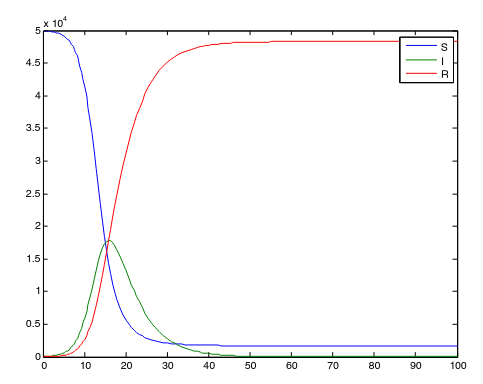
\includegraphics[width=\columnwidth]{Modelo SIR.png}
    \caption{Grafica de un Modelo SIR de un problema concreto \cite{weiss_2013}}
    \label{grafico modelo sir}
\end{figure}

En la figura \ref{grafico modelo sir} podemos apreciar una simulación calculada para un modelo matemático SIR determinado. Dentro de esta, podemos apreciar las tres ecuaciones que componen al modelo, y como estas cambiar a lo largo del tiempo.

\subsection{Modelo Matemático de SEIR}
\subsection{Modelo de Carga Potencial Máxima}

\subsection{Modelo de Gompertz}
El modelo de Gompertz, también llamado curva de Gompertz o función de Gompertz, es un modelo matemático para una serie temporal. La función es de tipo sigmoidea, y describe un crecimiento lengo en un periodo inicial y final, con uno más explosivo en un punto medio de la misma.

Inicialmente fue creada por Benjamin Gompertz para detallar su ley de la mortalidad humana, que se basa en un supuesto de que la resistencia de una persona a la muerte disminuye a medida que aumentan sus años, y fue descrito de la siguiente manera:

\begin{equation}
    N(t) = N(0) exp( -c ( exp(at) - 1))
\end{equation}

En esta ecuación, $N(t)$ representa un numero de individuos en un tiempo determinado $t$, por lo mismo, $N(0)$ representa la población inicial. $a$ denota una asíntota, $b$ y $c$ son valores positivos, que representan el desplazamiento a través del eje de las abcisas y la tasa de crecimiento, respectivamente. $exp$ denota la función exponencial.

\begin{figure*}
    \includegraphics[width=\textwidth]{casos diarios españa.png}
    \caption{Casos diarios de españa entre Marzo y Julio de 2020, fuente: cnecovid.isciii.es}
    \label{diarios españa}
\end{figure*}

En la publicación hecha por Sánchez-Villegas y colaboradores\cite{sanchez-villegas_codina_2020}, creada durante el año 2020, ellos decidieron utilizar el modelo de Gompertz para hacer una predicción del comportamiento de la epidemia de COVID-19 en España. Utilizando los datos de casos confirmados durante 47 días, generaron una curva de Gompertz que se ajustara lo más posible a sus datos.

¿Fue realmente acertado? Si bien, con la perspectiva inicial de dos años a futuro con respecto de esta publicación no lo parece para nada, contextualizando un poco a los datos que se tenían en ese momento podemos notar que la predicción fue, de hecho, relativamente acertada. En la figura \ref{diarios españa} podemos observar los casos diarios que se observan a lo largo del país entre las fechas de Marzo de 2020 hasta Julio del mismo año. La predicción inicial hecha por Sánchez-Villegas y colaboradores solo contemplaba datos hasta el 30 de abril de ese año, y contaba con solo 47 días de información, sin embargo, lograron demostrar que el pico de infección de españa llegó, efectivamente, en marzo de ese año, y que los contagios diarios iban extinguiendose.

Por desgracia, esta predicción cayó a mitades de Julio de 2020 y otras veces a futuro con la aparición de nuevas variantes y nuevos picos de infección en España y otros países del mundo. Aún así, el uso de este modelo predictivo en España y, según el autor, en la provincia de Hubei, donde ocurrió el primer caso de COVID, probó ser acertado para el corto plazo (Escala de Meses).
